%\documentclass[11pt]{report}
%\usepackage{siunitx}
%\usepackage{graphicx}

%\begin{document}
%\setcounter{chapter}{1}
%\tableofcontents


\newpage
\chapter{External stimulation methods, its effects and models}
This chapter delves into numerical models of external stimulation methods. Capacitive-coupled and direct-coupled external stimulation methods were considered for electric field stimulation delivery, while fluid flow-induced shear stress was considered for mechanical stimulation delivery. Reported biological effects and transducer pathways triggered by each stimulation method are also described. Finally, this chapter includes a state-of-the-art concise review on reported approaches for numerical modelling of each external stimulation method, including some case studies. 



\newpage
\section{Mechanical systems}
Several mechanical stimulation strategies have been developed in \ac{BTE} to overcome inhomogeneous cell distribution and suboptimal differentiation outcomes. In addition, these strategies aimed at accelerating bone formation processes \cite{Melke2018-kv}. Among the various developed mechanical stimulation setups \cite{Melo-Fonseca2023-fd}, fluid perfusion setups were selected for this thesis work, since these apply mechanical stimulation through fluid flow-induced wall shear stress while simultaneously performing mass transfer of nutrients and removal of cell metabolic waste. This is an advantage over other mechanical stimulation technologies operating on static cultures or closed containers without continuous culture medium replacement. This section enumerates the observed biological effects and proven underlying mechanisms for fluid flow-induced shear stress application for multiple cell lines. Literature-reported strategies for numerical modelling these mechanical setups are also discussed. 


\subsection{Fluid flow-induced shear stress setups}


\subsubsection{Reported biophysical effects}
Two categories of setups commonly apply flow-induced shear stress stimulation: the ones that generate a perfusion fluid flow \cite{McCoy2012-jv} and others that generate rotating fluid media (e.g., spinner flask, stirred tank bioreactor, rotating-wall vessel) \cite{Melke2018-kv}. Although both define specific ranges of wall shear stress, these also create dynamic conditions that are dependent on the fluid flow profile generated and pre-conditioned by several physical conditions (fluid velocity, turbulence, channel design, number of inlets and outlets, inserted scaffold design, etc.). If improperly planned and applied, they may result in cell detachment, damage, and apoptosis. Several setups for fluid-induced shear stress stimulation of cell-scaffold constructs have been developed over the years \cite{Alvarez-Barreto2011-lj, Filipowska2016-cd, Gardel2013-cs, Jaasma2008-oe}. Many differ significantly in design and protocol, which hinders precise comparisons and well-sustained identification of the effects of this type of mechanical stimulation in cells.

Biomechanical studies have demonstrated that more than 90\% of bone cells within the \ac{ECM} are osteocytes. These cells sense and transduce mechanical forces exerted on the bone, governing the rates of mineral resorption and deposition that occur during bone remodeling \cite{Franz-Odendaal2006-eu}. Mechanical stimulation applied to osteocytic networks under steady or oscillatory perfusion flow \cite{Lu2012-vh} is observed to modulate intracellular Ca\textsuperscript{2+} responses, specifically the calcium peak's magnitude and frequency, which vary with the fluid flow profiles. Effects of mechanical stimulation on \ac{MSCs} and their surrounding microenvironment were reviewed by Sun et al. \cite{Sun2022-xt}: mechanotransduction occurs via integrins and mechanosensitive ion channels that transmit the mechanical signals via actin stress fibers and known molecular pathways (e.g., RhoA, MAPK, Vinculin, Talin, ERK, YAP/TAZ). Interestingly, some stretch-activated channels mediate intracellular Ca\textsuperscript{2+} responses upon mechanical stimulation \cite{Walker2000-bc, Luo2013-wv}, an effect also showed to be induced by \acs{AC} electric fields in this type of channels in the absence of mechanical stimulation \cite{Cho1999-hr}, which indicates the potential for these channels to be modulated for both kinds of biophysical stimulation. Also, the Wnt signaling pathway was observed to be an essential control mechanism in bone response to mechanical loading \cite{Choi2021-jk}. \ac{MSCs}, when subjected to fluid flow-induced wall shear stress, showed an increase in cell attachment, spreading, cell viability, and osteogenic differentiation \cite{De_Luca2020-hp}. This is transduced in the expression of early markers of osteogenic differentiation like \acs{RUNX2}, \ac{ALP}, and osteopontin or \ac{SPP1}, as well as increased mineralization, comparatively to a static culture. The mechanical environment of bone is complex, and it remains unclear how precisely macro-scale mechanical actions will translate into micro-scale events that regulate and affect bone precursor cell differentiation. Nevertheless, mechanical stimulation has been shown to promote bone growth, improving mineralization and secretion of many specialized extracellular matrix proteomes, such as type I collagen \cite{Partap2010-xt}.


\subsubsection{Reported numerical modelling techniques}
Numerically modelling perfusion setups with or without porous scaffolds requires virtualizing their physical structures. This step can be accomplished in multiple ways, either by drawing their equivalent \ac{CAD} geometries or by obtaining their physical structure from image acquisition techniques (e.g., \ac{mCT}), followed by a subsequent tridimensional reconstruction. Fluid flow modelling is usually obtained by solving continuity and \ac{3D} Navier Stokes equations on these complex geometries. If the scaffold is present, no-slip wall conditions are considered for all physical boundaries, including the scaffold surface. The culture medium is modeled as an incompressible Newtonian fluid, and the solution to all this set of equations is obtained by computational methods, namely by \ac{FEM} \cite{Campos_Marin2018-ff, McCoy2012-jv, Vis2023-xt} or by the \ac{FVM} \cite{De_Wildt2023-ev}. When the geometry of the scaffold's porosity is unknown, it is expected to introduce a new set of equations that account for a global permeability, as determined by Darcy's law \cite{De_Wildt2023-ev}. Empirical models have also been developed to calculate the fluid-induced wall shear stress \cite{Ahmed2023-es}, offering an alternative to the solution obtained from \ac{CFD} techniques that use the resultant shear rate and the fluid kinematic viscosity to perform that calculation. In Chapter 3, \ac{CFD} techniques are used to understand the impact of bioreactor design changes in delivering fluid-induced shear stress to the cultured cells region.



\section{Electromagnetic systems}
The two most important communicating systems in the human body, affecting cellular functions, are the nervous and hormonal systems. These two systems act mainly on the cell's membranes to induce endogenous \ac{EF}s that modulate interactions between intracellular and extracellular environments. As macroscopic functions of the body have been reported to be affected by an applied external electric field, it is straightforward to hypothesize that cellular membrane signal transduction mechanisms can be modulated by an applied \ac{EF} of specific strength and form \cite{Seegers2001-jo}.

Multiple experimental setups have been developed and applied to deliver electromagnetic stimulation to \textit{in vitro} cell cultures in \ac{BTE}. A significant number of reviews split electromagnetic applying experimental setups into a subset of technologies, according to the different aspects of how they obtain the electric and/or magnetic field that will exert an effect on the cell culture \cite{Thrivikraman2018-su, Funk2009-is}. As was presented in the previous chapter, \ac{DCoupled} and \ac{CCoupled} systems were selected for further analysis in this work due to their capability to apply isolated \ac{EF}s. The treatment of \textit{in vitro} cell cultures with \ac{EF}s can evoke biochemical and physiological responses that can be favorable to \ac{BTE} outcomes, provided that the stimulation parameters (e.g., waveform signal, exposure duration, field strength, frequency) are within tolerance limits for the exposed cellular type. Despite multiple evidence of the biological effects produced by cell culture exposure to an \ac{EF}, the complete mechanism of this interaction remains unknown, strongly limiting the accuracy of the applications of \ac{EFs} based therapies \cite{Taghian2015-hf}.

\textit{In vitro} and \textit{in vivo} reports commonly attribute the observed \ac{EF} effects to the activation of membrane proteins, specifically proteins involved in signal-transduction mechanisms. Particularly, the concentration of free cytosolic Ca\textsuperscript{2+} is observed to follow the electric stimulation of cells, contributing to activate a cascade of calcium-dependent cellular processes \cite{Pall2013-wt, De_Menorval2016-fv, Brighton2001-fk, Burke2017-su, Cho1999-hr} including cellular motility \cite{Onuma1988-eu}, redistribution of integral membrane proteins and reorganization of microfilament structures \cite{Cho1999-hr}. The oscillation of intracellular free cytosolic calcium concentration is significant for cell signaling and is reported to be impacted by electromagnetic stimulation \cite{Sun2007-tx}. This oscillation is a complex dynamical process and reflects calcium transportation to and from the exterior cell, cytosol, intracellular stores, exchange between cells, or diffusion and buffering due to its binding to proteins. According to Sun et al. \cite{Sun2007-tx}, regulating calcium oscillation by external physical stimulation could amplify \ac{MSCs} differentiation into a tissue-specific lineage and may offer alternative biotechnology to harness the unique properties of stem cells. Osteogenic markers impacted by electromagnetic stimulation include the expression of \acs{ALP}, \acs{COL1}, osteocalcin and osteopontin, BMP-2, DCN, \acs{RUNX2}, MAPK, ERK, p38 \cite{Guillot-Ferriols2022-wn}. An extensive list of osteogenic differentiation regulatory agents was compiled by Deng et al. \cite{Deng2008-xs}, and a review of the positive and negative effects of electromagnetic stimulation in stem cells is given by Maziarz \textit{et al.} \cite{Maziarz2016-fd}. This section enumerates the observed biological effects and underlying mechanisms for \ac{DCoupled} and \ac{CCoupled} systems. It also discusses the impact of different \ac{EF} patterns applied by both systems in specific cellular responses and how particular setup characteristics contribute to this impact \cite{Meng2021-qn}.


\subsection{Direct-coupled setups}


\subsubsection{Reported biophysical effects}
\textit{In vitro} \ac{DCoupled} electric field stimulation is applied through electrodes immersed in a culture medium, or using a conductive surface/scaffold or Agar-salt bridges \cite{Meng2013-mz}. Direct-current (\acs{DC}) signals are one of the most applied, being current or voltage-controlled. Other studies apply alternate-current (\acs{AC}) or pulsed signals to charge-balance the culture medium, mitigating one of the DCoupled drawbacks, which is a rising gradient in ion distribution in the culture medium that results in altered cell physiology, thus making it difficult to distinguish the effects occurring due to electric field stimulation \cite{Meng2021-qn}. Although variable in the magnitude, frequency, exposure, and waveform, \ac{DCoupled} \ac{EF} stimulation has sequentially proven to modulate different phases of the cell cycle and their metabolic processes, impacting cell proliferation, morphology, and differentiation. 

When subjected to \ac{DCoupled} stimulation, \acs{MSCs} proliferation and osteogenic differentiation occur, accompanied by cell membrane potential changes, with membrane depolarization corresponding to the proliferative phase and membrane hyperpolarization corresponding to the differentiative phase \cite{Bhavsar2019-iz}. Modulation of \acs{MSCs} biomechanics through electrical influence on the cytoskeleton elasticity was observed by Titushkin \textit{et al.} \cite{Titushkin2009-gi}, where elasticity was reduced due to substantial actin reorganization and led to changes in specific linker proteins (ezrin/radixin/moesin family) at focal adhesion sites. These morphological modifications are hypothesized to be connected to the control of cell differentiation and other cellular processes that can, by this way, become efficiently regulated by a \acs{DCoupled} electrical stimulus.

Osteoblast-like cells subjected to \acs{DCoupled} stimulation \cite{Wang1998-ek} increased their proliferation and the presence of calcification deposits. Intracellular free calcium ion concentration was measured, showing an average increase of 2.3 times the initial level. This intracellular calcium ion concentration effect was also observed in \ac{MSCs} cultured in silk scaffold \cite{Cakmak2016-oj} and in conductive scaffolds \cite{Zhang2016-ul} when subjected to a \acs{DCoupled} stimulation. Also, \acs{MSCs} seeded into conductive scaffolds subjected to \acs{DCoupled} stimulation together with blockers of voltage-gated calcium (Ca\textsuperscript{2+}\textsubscript{v}), sodium (Na\textsuperscript{+}\textsubscript{v}), potassium (K\textsuperscript{+}\textsubscript{v}), or chloride (Cl\textsuperscript{-}\textsubscript{v}) channels, showed stimulation reduced effects with the presence of Na\textsuperscript{+}\textsubscript{v}, K\textsuperscript{+}\textsubscript{v}, or Cl\textsuperscript{-}\textsubscript{v} blockers and completely nullified effects with Ca\textsuperscript{2+}\textsubscript{v} blocker. These results indicate that ion fluxes through these channels are promoted by \acs{DCoupled} stimulation and that Ca\textsuperscript{2+}\textsubscript{v} channels play a more critical role than the other three tested channels \cite{Zhang2016-ul}. Another study \cite{Kim2009-dv} reports that applying \acs{DCoupled} stimulation through a biphasic waveform to \acs{MSCs} increased proliferation, alkaline phosphatase activity, calcium deposition, vascular endothelial growth factor and
BMP-2 production. Treatment with selective inhibitors of p38, MAPK, or ERK, as well as calcium channel blockers, reduced the increase
of vascular endothelial growth factor expression and cell proliferation. Kim \textit{et al.} \cite{Kim2009-dv} point that osteoblast differentiation of hMSCs occurs by enhancement of cell proliferation and modulation of the local endocrine environment through \ac{VEGF} and BMP-2, inducing the activation of MAPK (ERK and p38) and the calcium channel.

Studies that applied electric fields in \ac{BTE} research throughout \ac{DCoupled} setups report positive effects for a broad range of \ac{EF} magnitudes, as shown in Figure \ref{fig: F2d1}. Despite the considerable applicability of \ac{DCoupled} stimulation as a tool to improve \ac{BTE} solutions, a systematic study of the impact of the \ac{EF}, with an improved understanding of underlying biochemical mechanisms that are activated, is still missing to optimize its application outcomes. \ac{DCoupled} electric fields were observed to influence different phases of the cellular cycle, from differentiation to proliferation and maturation in terms of late-stage gene expression and development of osteogenic-phenotype properties. However, depending on the type of metals used in \ac{DCoupled} systems' electrodes, an irreversible metal dissolution might occur, modifying the \ac{pH} value of the medium, an undesired effect that may go along with electrode corrosion provoking cytotoxic effects. Faradaic by-products resulting from redox and electrochemical reactions at the electrode-electrolyte interface (carbon reactions, water chemistry interactions) can mislead the results from the application of \ac{EF}s, unless a profound characterization of the electrode-electrolyte interface environment is taken into consideration \cite{Spadaro1982-af}. \ac{DCoupled} systems using salt bridges successfully circumvent this limitation, but present other disadvantages related to the small area of charge delivery, the presence of cell diffusion effects due to concentration differences between bridge contents and culture medium, and difficulties in running several chambers simultaneously while maintaining a stable reaction rate \cite{Guette-Marquet2021-rp}.


\begin{figure}
\makebox[\textwidth][c]{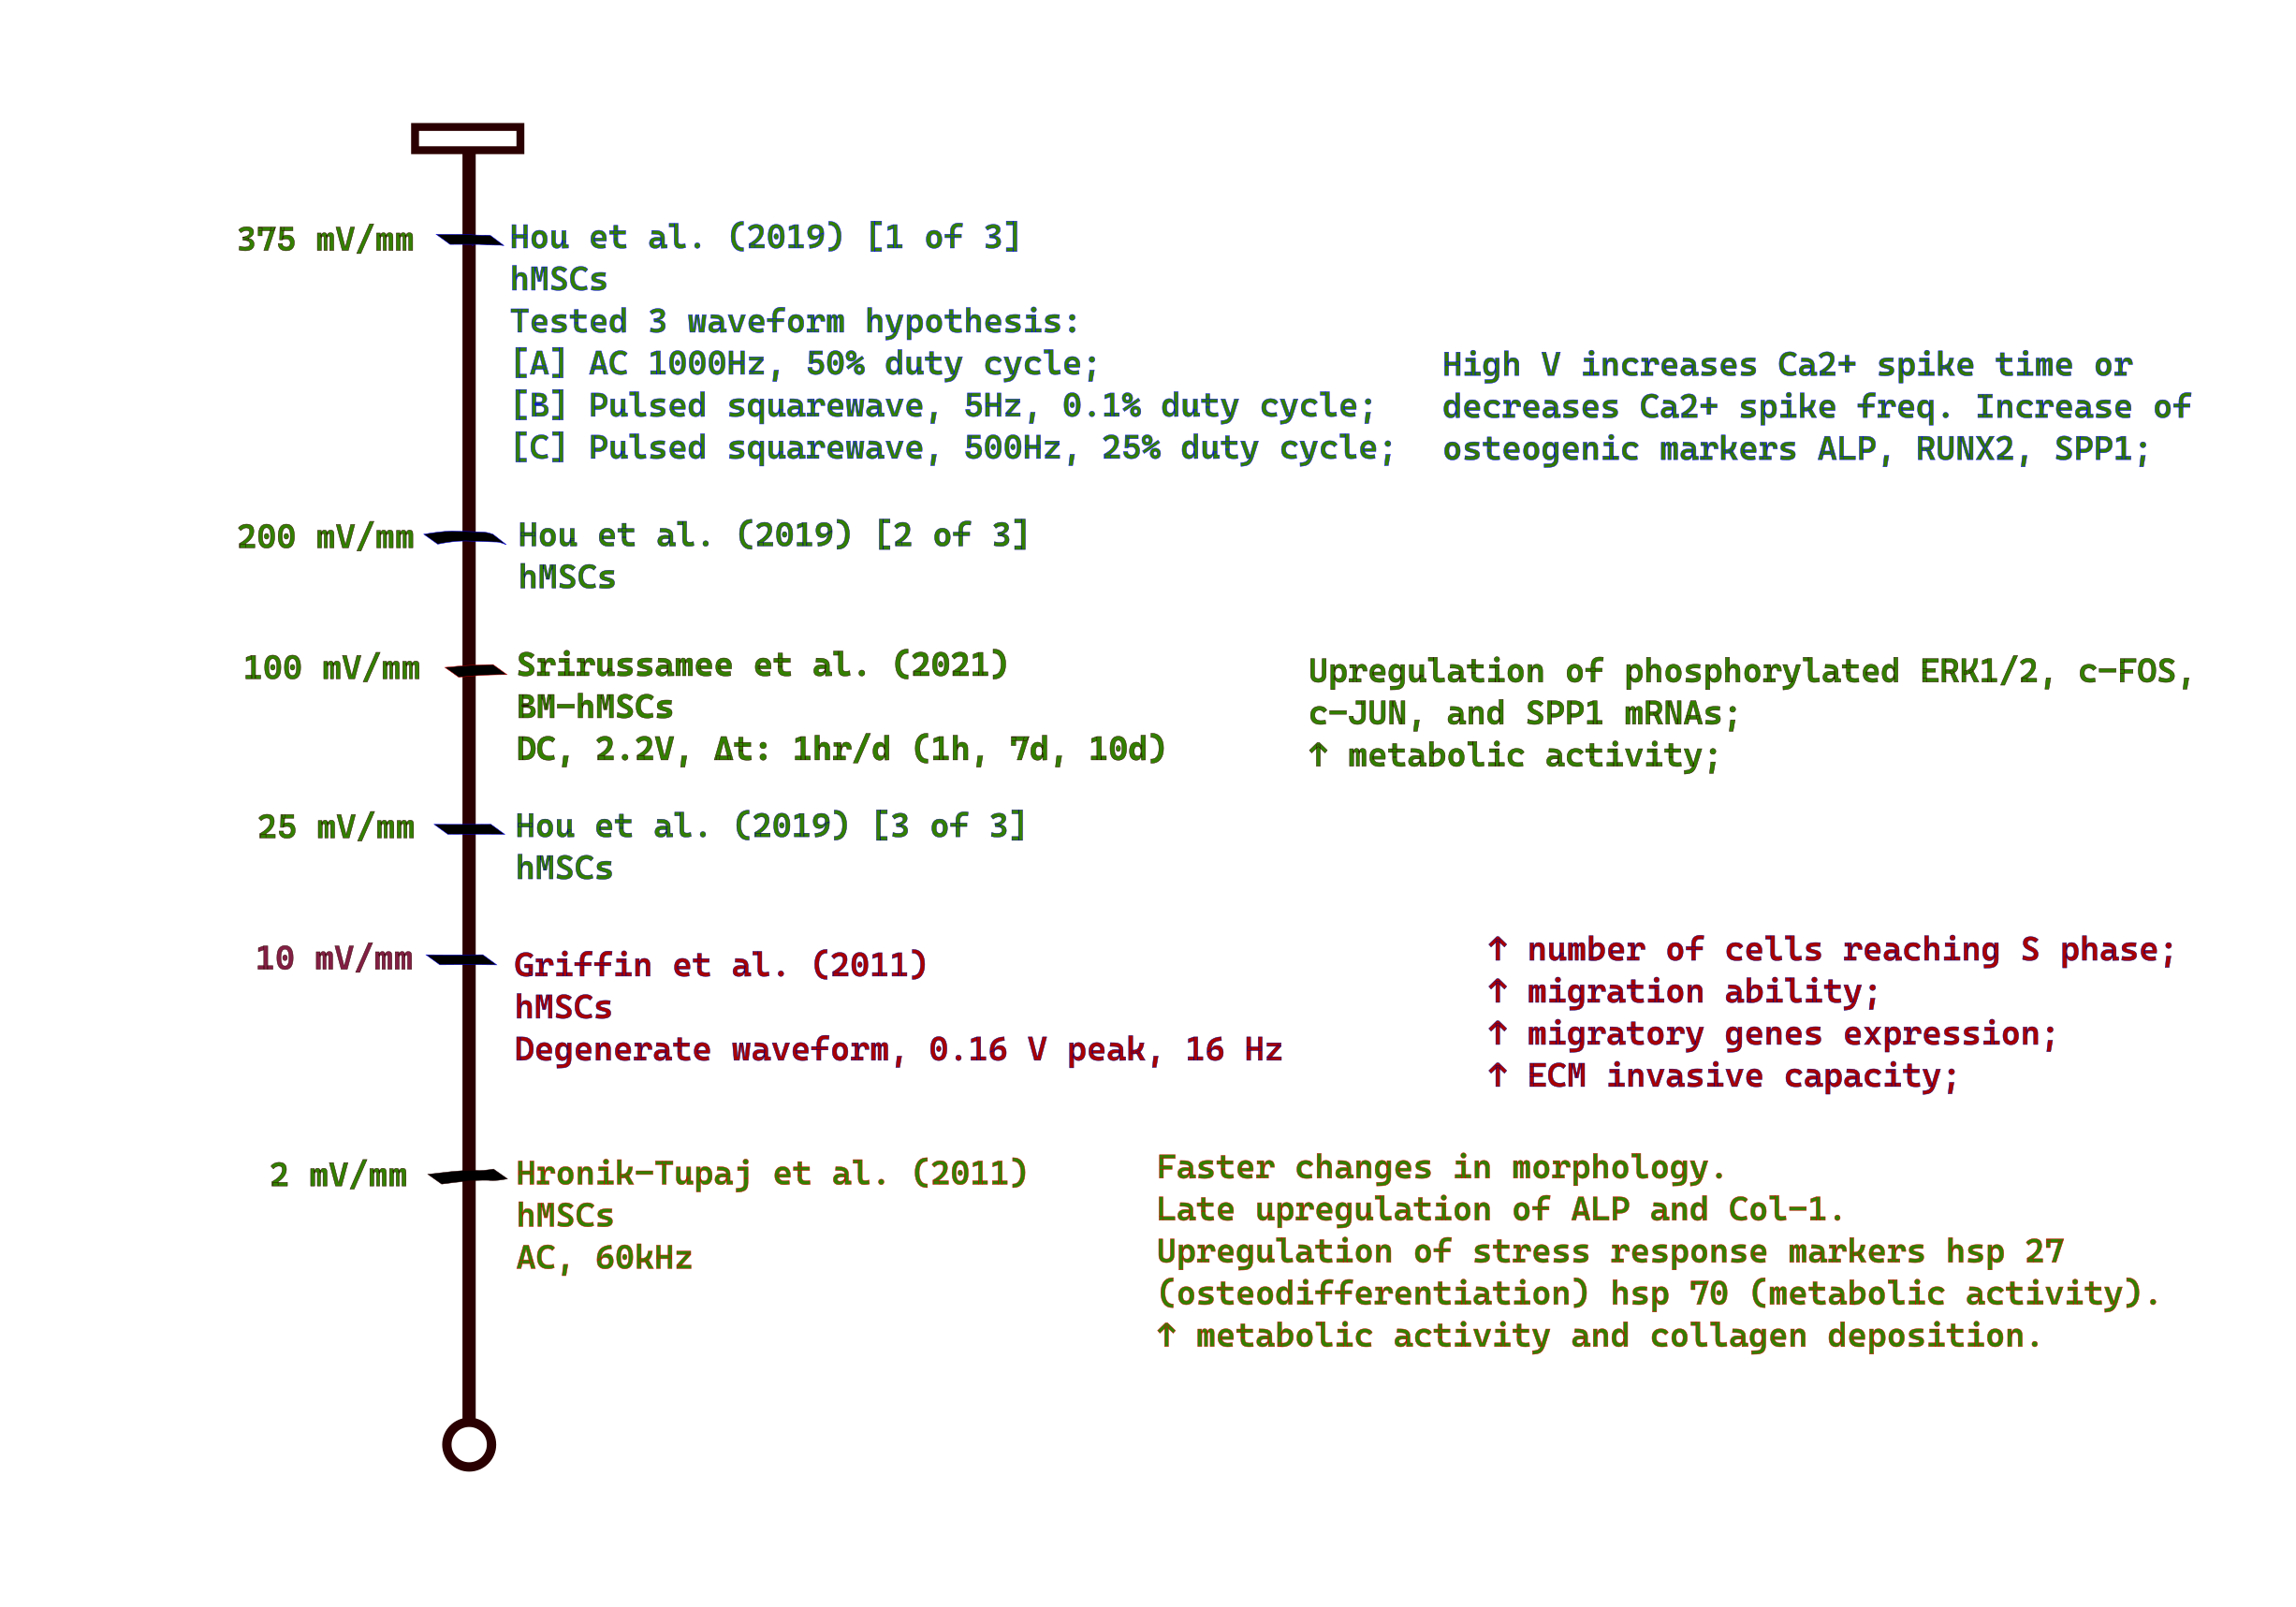
\includegraphics[scale=0.3]{./figures/Figure_2d1.png}}
\caption{A sample of reported electric field magnitudes and biological effects for the same exposed cell type (hMSCs) in different Dcoupled (green) and CCoupled (red) systems.}
\label{fig: F2d1}
\end{figure}
      

\subsubsection{Reported numerical modelling techniques}
Experimentally obtained \ac{DCoupled} \ac{EF} ranges that promote specific cellular processes may be found for several cell types and metabolic phases. Still, the diversity of applied protocols and system options prevents an effective comparison and the drawing of global conclusions. Numerical modelling techniques have been introduced to \ac{DCoupled} systems to help to understand and control the effective magnitude of \ac{EF} stimulation being applied and to get hints on the most probable intracellular targets of a particular stimulation protocol. 

Approaches found in the literature use analytical estimates to predict the \ac{EF} magnitude delivered by DCoupled systems. These divide the applied potential by the distance between the electrodes \cite{Mobini2016-jh} or use adaptations of Gauss’s Law to calculate the electric field strength at any distance \cite{Hronik-Tupaj2011-cx}. More complex \ac{FEM}-based approaches were applied to model \ac{DCoupled} systems, considering the entire tridimensional reality of the setup. A \ac{FEM} computational model using a set of electrochemistry equations was established by Srirussamee \textit{et al.} \cite{Srirussamee2021-cj}, considering a secondary current distribution to calculate the transport of charged ions in an electrolyte, while using the Butler-Volmer equation to include activation overpotentials, charge transfer reactions and Ohm's law to include the electrodes conduction with a charge balance. With increased complexity, this last model tries to introduce the electrode/electrolyte interface dynamics, improving the existing analytical alternatives. A different \ac{FEM} approach used a quasi-static approximation of Maxwell’s equations \cite{Stephan2020-qh, Shaner2023-on, Zimmermann2021-fx}, considering Laplace’s equation to solve for the electric potential, and including Ohm's law with a set of equations to guarantee electric field irrotational conditions and the conservation of electric currents. This last \ac{FEM} modelling strategy can be used on its own or can be combined with electrode/electrolyte experimental characterization data to develop a reliable dose-response curve for the delivery of an electric field or current in a \ac{DCoupled} system \cite{Zimmermann2023-gm}. Similar to this last modelling proposition, a combined approach between an experimental electric current measurement and a \ac{FEM} implementation of electric currents equations was applied and is described in Chapter 4 to model a \ac{DCoupled} system, introducing the electrode/electrolyte effects by indirectly employing the resultant current.  


\subsection{Capacitive-coupled setups}


\subsubsection{Reported biophysical effects}
In \ac{BTE}, \textit{in vitro} \ac{CCoupled} electric field stimulation is one of the oldest stimulation processes applied to promote bone cell activity. Usually, at \ac{CCoupled} setups, the electrodes are placed in parallel positions (despite not being mandatory), and they are separated from the culture medium by an air gap or an electrical insulator material. This separation forms a capacitor that accumulates surface charges when a potential is applied, creating an \ac{EF} between the electrodes \cite{Thrivikraman2018-su}. The insulator barrier present in \ac{CCoupled} systems prevents the generation of faradaic byproducts and electrode corrosion reactions. The applied waveform signal must contain high-frequency components to surpass this conductivity barrier and guarantee that an effective electric field reaches the cellular content. This constitutes one drawback of \ac{CCoupled} systems, since the voltage drop across the culture medium is only a tiny fraction of the applied voltage, i.e., the \ac{EF} induced in the culture medium is weak when compared to that obtained by \ac{DCoupled} setups. However, the efficiency of capacitive coupling increases with frequency. So, the strength of the induced \ac{EF} can be increased by working at higher frequencies as an alternative to applying higher voltages. Differences in electrical conductivities between the insulator and culture medium (and any other material present in the culture) will impact the spatial and temporal profile of the generated \ac{EF}. \ac{CCoupled} applications are known to generate non-faradaic processes, like the build-up of capacitive ion storage in an electric double layer, ion kinetics modifications related to ion mobility, and the creation of chemical surface charges.

A diverse range of \ac{EF} magnitudes, frequencies, and input waveforms (sinusoidal, pulsed square, asymmetric sawtooth, degenerate wave) have been applied by different \ac{CCoupled} setups \cite{Brighton1992-gg, Hartig2000-ny, Korenstein1984-qb}, obtaining favorable effects in bone line cells like proliferation, differentiation, extracellular matrix maturation, and mineralization. \ac{CCoupled} \ac{EF}s source of effects is attributed to polarization mechanisms that directly provoke the activation of membrane proteins and/or generate ion flux displacements, in both differentiated and undifferentiated cells \cite{Korenstein1984-qb, Danon1984-eu, Ozawa1989-uz}. Secondary messengers are known to be involved in transducing \ac{CCoupled} stimulation into cellular effects. \ac{CCoupled} stimulation is known to upregulate cyclic adenosine monophosphate, involved in the activation of protein kinases, which in turn favor \acs{DNA} transcription to initiate cell division \cite{Korenstein1984-qb}. Calcium uptake was observed to increase after \ac{CCoupled} stimulation \cite{Danon1984-eu}, activating the signaling cascades necessary for proliferation and differentiation, like the calmodulin pathway. The calcium transduction pathway was observed to occur through cellular membrane voltage-gated calcium channels or the release from cellular internal reservoirs, such as the endoplasmic reticulum \cite{Clark2014-sz, Brighton2001-fk}. Another set of observations showed that \ac{CCoupled} stimulation provokes cytoskeleton changes evidenced by actin polymerization \cite{Laub1984-qm, Binderman1984-og}. \acs{ALP} enzyme is involved in dephosphorylating processes essential for macromolecule syntheses, such as \ac{HA} and other components of bone \ac{ECM}. \acs{ALP} upregulation was observed to be promoted by \ac{CCoupled} stimulation and is followed by the increase of bone phenotypes maturation markers, like \acs{BMP} and \acs{TGF}, increasing the repair and upregulation of bone differentiation markers \cite{Clark2014-sz, Wang2006-hx}. Mineralization is observed to increase after more extended periods applying \ac{CCoupled} stimulation.    


\subsubsection{Reported numerical modelling techniques}
Numerical modelling of \ac{CCoupled} setups applying \ac{EF} stimulation protocols has been developed to predict and understand the \ac{EF} strength being applied. An existing approach to model \acs{CCoupled} systems is to consider a circuit in parallel comprising both resistor and capacitor elements \cite{Hartig2000-ny, Korenstein1984-qb}, and solve it analytically to find the electric potential drop in the cell culture medium. Another approach solves Maxwell’s electromagnetic field equations using \acs{FEM} techniques \cite{Brighton1992-gg, Armstrong1988-ob, Stephan2020-qh}, considering appropriate boundary conditions, resulting in a \ac{3D} computer-generated solution. The diversity of stimulation parameters applied in the \acs{CCoupled} studies (e.g., magnitude, frequency, duty cycle, waveform) raises questions regarding the most relevant \ac{EF} characteristics to modulate a particular osteogenic response. In Chapter 5, multiple modelling techniques were applied to diverse \ac{CCoupled} setups reported in the literature to identify the agreement between different modelling strategies that predict \ac{EF}, ultimately comparing with the value reported for each \textit{in vitro} setup.
  


\section{Summary}
\ac{EF} transduction and mechanotransduction depend on cell type maturation and differentiation phase since they express different membrane channel proteins at each development stage, among other phenotype properties. Cells privilege specific metabolic pathways according to their evolution and their surroundings. Considerable evidence collected and reviewed demonstrates that external stimulation impacts cellular mechanisms, providing a way to interfere with proliferation, cell functions, and differentiation outcomes. However, due to significant methodological differences between existent studies, it is challenging to draw comparisons and conclusions about all the involved cellular pathways. Although it is possible to hypothesize that they all can play a part in transducing external stimulation signals, understanding and weighing the importance of each pathway may be crucial to developing external stimulation systems and protocols toward more optimized outputs. This thesis hypothesizes that to make sense of the biological stimulation effects, it is first necessary to determine the conditions generated in the cell culture region by each type of external stimulation. This will be addressed in the following three chapters for different stimulation experimental setups with different stimulation protocol paradigms, using numerical modelling to predict the stimulation conditions being applied. Finally, in Chapter 6, the conclusions from each studied setup technology will be brought together into a data-driven strategy based on numerical predictions to design a multimodal bioreactor able to deliver precise and replicable stimulation ranges. 



%\newpage
%\bibliography{library_c2} 
%\bibliographystyle{plain}
%\end{document}